\documentclass[12pt]{article}
\usepackage{tikz}
\usepackage{amsmath}
% Underlining package
\usepackage{ulem}
\usetikzlibrary{calc}
\usetikzlibrary{angles,quotes}
\usepackage[a4paper, portrait, margin=1cm]{geometry}
\usepackage{fancyhdr}

\newcommand{\HeadingQuestions}{%
\section*{\Large Name: \underline{\hspace{8cm}} \hfill Date: \underline{\hspace{3cm}}}%
\vspace{-3mm}\par
\textbf{Area Squares}\vspace{1pt}\hrule
}

% raise footer with page number; no header
\fancypagestyle{myfancypagestyle}{
  \fancyhf{}% clear all header and footer fields
  \renewcommand{\headrulewidth}{0pt} % no rule under header
  \fancyfoot[C] {\thepage} \setlength{\footskip}{14.5pt} % raise page number allowed min 14.5pt
}
\pagestyle{myfancypagestyle}  % apply myfancypagestyle

\newcounter{minipagecount}

\begin{document}
\HeadingQuestions
\vspace{8mm}

\begin{minipage}{0.55\textwidth}
  \refstepcounter{minipagecount}
  \noindent{(\theminipagecount)}\quad
  \begin{tikzpicture}[scale=1.1, baseline=(current bounding box.north)]
    \begin{scope}[rotate=0]
        % Draw square
        \draw (0,0) coordinate (A) --
              ++(2.076,0) coordinate (B) --
              ++(0,2.076) coordinate (C) --
              ++(-2.076,0) coordinate (D) -- cycle;

        % Right angle markers
        \foreach \p/\q/\r in {D/A/B,A/B/C,B/C/D,C/D/A} {
            \pic [draw, -, angle radius=0.2cm] {right angle=\p--\q--\r};
        }

        % Vertex LABELS
        % Labels relative to shape geometry
        \node at ($(A)+(-0.2,-0.2)$) {A};
        \node at ($(B)+(0.2,-0.2)$) {B};
        \node at ($(C)+(0.2,0.2)$) {C};
        \node at ($(D)+(-0.2,0.2)$) {D};

        % Tick marks across horizontal sides
        \draw[thin, gray]
            ($(A)!0.5!(B) + (0,-0.10)$) --
            ($(A)!0.5!(B) + (0,0.10)$);

        \draw[thin, gray]
            ($(D)!0.5!(C) + (0,-0.10)$) --
            ($(D)!0.5!(C) + (0,0.10)$);

        % Tick marks across vertical sides
        \draw[thin, gray]
            ($(B)!0.5!(C) + (-0.10,0)$) --
            ($(B)!0.5!(C) + (0.10,0)$);

        \draw[thin, gray]
            ($(A)!0.5!(D) + (-0.10,0)$) --
            ($(A)!0.5!(D) + (0.10,0)$);


        % dotted/dashed arrows shifted away from edges
        % % Vertical side (B-C), shifted right
        \draw[<->, gray]
            ($(B) + (0.45cm,0)$) -- ($(C) + (0.45cm,0)$)
            node[black, midway, fill=white, xshift=2mm, inner sep=3pt] {7\,cm};

    \end{scope}
\end{tikzpicture}
\end{minipage}%
\hfill
\begin{minipage}{.4\textwidth}
  \begin{align*}
  \text{Area} &= l^2 \\
  \text{Area} &= \dotuline{~~~~~~~} \,\text{cm} \times \dotuline{~~~~~~~} \,\text{cm} \\
  \text{Area} &= \dotuline{~~~~~~~} \,\text{cm}^2
  \end{align*}
\end{minipage}
\par\vspace{1cm}\begin{minipage}{0.55\textwidth}
  \refstepcounter{minipagecount}
  \noindent{(\theminipagecount)}\quad
  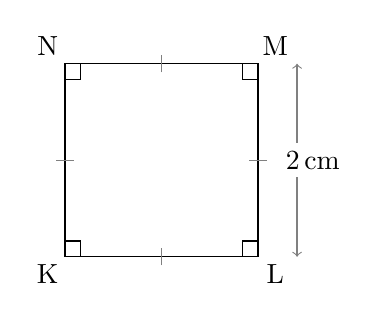
\begin{tikzpicture}[scale=1.1, baseline=(current bounding box.north)]
    \begin{scope}[rotate=0]
        % Draw square
        \draw (0,0) coordinate (K) --
              ++(2.229,0) coordinate (L) --
              ++(0,2.229) coordinate (M) --
              ++(-2.229,0) coordinate (N) -- cycle;

        % Right angle markers
        \foreach \p/\q/\r in {N/K/L,K/L/M,L/M/N,M/N/K} {
            \pic [draw, -, angle radius=0.2cm] {right angle=\p--\q--\r};
        }

        % Vertex LABELS
        % Labels relative to shape geometry
        \node at ($(K)+(-0.2,-0.2)$) {K};
        \node at ($(L)+(0.2,-0.2)$) {L};
        \node at ($(M)+(0.2,0.2)$) {M};
        \node at ($(N)+(-0.2,0.2)$) {N};

        % Tick marks across horizontal sides
        \draw[thin, gray]
            ($(K)!0.5!(L) + (0,-0.10)$) --
            ($(K)!0.5!(L) + (0,0.10)$);

        \draw[thin, gray]
            ($(N)!0.5!(M) + (0,-0.10)$) --
            ($(N)!0.5!(M) + (0,0.10)$);

        % Tick marks across vertical sides
        \draw[thin, gray]
            ($(L)!0.5!(M) + (-0.10,0)$) --
            ($(L)!0.5!(M) + (0.10,0)$);

        \draw[thin, gray]
            ($(K)!0.5!(N) + (-0.10,0)$) --
            ($(K)!0.5!(N) + (0.10,0)$);


        % dotted/dashed arrows shifted away from edges
        % % Vertical side (B-C), shifted right
        \draw[<->, gray]
            ($(L) + (0.45cm,0)$) -- ($(M) + (0.45cm,0)$)
            node[black, midway, fill=white, xshift=2mm, inner sep=3pt] {2\,cm};

    \end{scope}
\end{tikzpicture}
\end{minipage}%
\hfill
\begin{minipage}{.4\textwidth}
  \begin{align*}
  \text{Area} &= l^2 \\
  \text{Area} &= \dotuline{~~~~~~~} \,\text{cm} \times \dotuline{~~~~~~~} \,\text{cm} \\
  \text{Area} &= \dotuline{~~~~~~~} \,\text{cm}^2
  \end{align*}
\end{minipage}
\par\vspace{1cm}\begin{minipage}{0.55\textwidth}
  \refstepcounter{minipagecount}
  \noindent{(\theminipagecount)}\quad
  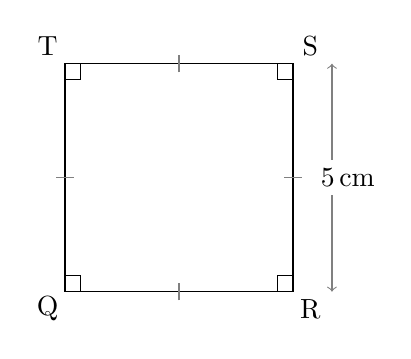
\begin{tikzpicture}[scale=1.1, baseline=(current bounding box.north)]
    \begin{scope}[rotate=0]
        % Draw square
        \draw (0,0) coordinate (Q) --
              ++(2.632,0) coordinate (R) --
              ++(0,2.632) coordinate (S) --
              ++(-2.632,0) coordinate (T) -- cycle;

        % Right angle markers
        \foreach \p/\q/\r in {T/Q/R,Q/R/S,R/S/T,S/T/Q} {
            \pic [draw, -, angle radius=0.2cm] {right angle=\p--\q--\r};
        }

        % Vertex LABELS
        % Labels relative to shape geometry
        \node at ($(Q)+(-0.2,-0.2)$) {Q};
        \node at ($(R)+(0.2,-0.2)$) {R};
        \node at ($(S)+(0.2,0.2)$) {S};
        \node at ($(T)+(-0.2,0.2)$) {T};

        % Tick marks across horizontal sides
        \draw[thin, gray]
            ($(Q)!0.5!(R) + (0,-0.10)$) --
            ($(Q)!0.5!(R) + (0,0.10)$);

        \draw[thin, gray]
            ($(T)!0.5!(S) + (0,-0.10)$) --
            ($(T)!0.5!(S) + (0,0.10)$);

        % Tick marks across vertical sides
        \draw[thin, gray]
            ($(R)!0.5!(S) + (-0.10,0)$) --
            ($(R)!0.5!(S) + (0.10,0)$);

        \draw[thin, gray]
            ($(Q)!0.5!(T) + (-0.10,0)$) --
            ($(Q)!0.5!(T) + (0.10,0)$);


        % dotted/dashed arrows shifted away from edges
        % % Vertical side (B-C), shifted right
        \draw[<->, gray]
            ($(R) + (0.45cm,0)$) -- ($(S) + (0.45cm,0)$)
            node[black, midway, fill=white, xshift=2mm, inner sep=3pt] {5\,cm};

    \end{scope}
\end{tikzpicture}
\end{minipage}%
\hfill
\begin{minipage}{.4\textwidth}
  \begin{align*}
  \text{Area} &= l^2 \\
  \text{Area} &= \dotuline{~~~~~~~} \,\text{cm} \times \dotuline{~~~~~~~} \,\text{cm} \\
  \text{Area} &= \dotuline{~~~~~~~} \,\text{cm}^2
  \end{align*}
\end{minipage}
\par\vspace{1cm}\begin{minipage}{0.55\textwidth}
  \refstepcounter{minipagecount}
  \noindent{(\theminipagecount)}\quad
  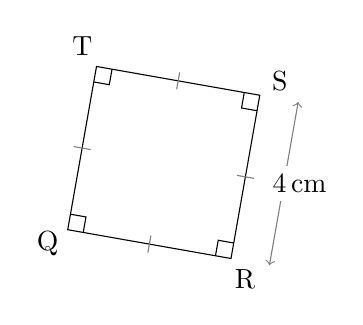
\begin{tikzpicture}[scale=1.1, baseline=(current bounding box.north)]
    \begin{scope}[rotate=-10]
        % Draw square
        \draw (0,0) coordinate (Q) --
              ++(1.914,0) coordinate (R) --
              ++(0,1.914) coordinate (S) --
              ++(-1.914,0) coordinate (T) -- cycle;

        % Right angle markers
        \foreach \p/\q/\r in {T/Q/R,Q/R/S,R/S/T,S/T/Q} {
            \pic [draw, -, angle radius=0.2cm] {right angle=\p--\q--\r};
        }

        % Vertex LABELS
        % Labels relative to shape geometry
        \node at ($(Q)+(-0.2,-0.2)$) {Q};
        \node at ($(R)+(0.2,-0.2)$) {R};
        \node at ($(S)+(0.2,0.2)$) {S};
        \node at ($(T)+(-0.2,0.2)$) {T};

        % Tick marks across horizontal sides
        \draw[thin, gray]
            ($(Q)!0.5!(R) + (0,-0.10)$) --
            ($(Q)!0.5!(R) + (0,0.10)$);

        \draw[thin, gray]
            ($(T)!0.5!(S) + (0,-0.10)$) --
            ($(T)!0.5!(S) + (0,0.10)$);

        % Tick marks across vertical sides
        \draw[thin, gray]
            ($(R)!0.5!(S) + (-0.10,0)$) --
            ($(R)!0.5!(S) + (0.10,0)$);

        \draw[thin, gray]
            ($(Q)!0.5!(T) + (-0.10,0)$) --
            ($(Q)!0.5!(T) + (0.10,0)$);


        % dotted/dashed arrows shifted away from edges
        % % Vertical side (B-C), shifted right
        \draw[<->, gray]
            ($(R) + (0.45cm,0)$) -- ($(S) + (0.45cm,0)$)
            node[black, midway, fill=white, xshift=2mm, inner sep=3pt] {4\,cm};

    \end{scope}
\end{tikzpicture}
\end{minipage}%
\hfill
\begin{minipage}{.4\textwidth}
  \begin{align*}
  \text{Area} &= l^2 \\
  \text{Area} &= \dotuline{~~~~~~~} \,\text{cm} \times \dotuline{~~~~~~~} \,\text{cm} \\
  \text{Area} &= \dotuline{~~~~~~~} \,\text{cm}^2
  \end{align*}
\end{minipage}
\par\vspace{1cm}\begin{minipage}{0.55\textwidth}
  \refstepcounter{minipagecount}
  \noindent{(\theminipagecount)}\quad
  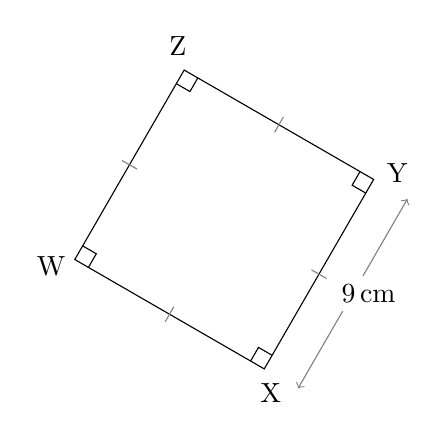
\begin{tikzpicture}[scale=1.1, baseline=(current bounding box.north)]
    \begin{scope}[rotate=-30]
        % Draw square
        \draw (0,0) coordinate (W) --
              ++(2.526,0) coordinate (X) --
              ++(0,2.526) coordinate (Y) --
              ++(-2.526,0) coordinate (Z) -- cycle;

        % Right angle markers
        \foreach \p/\q/\r in {Z/W/X,W/X/Y,X/Y/Z,Y/Z/W} {
            \pic [draw, -, angle radius=0.2cm] {right angle=\p--\q--\r};
        }

        % Vertex LABELS
        % Labels relative to shape geometry
        \node at ($(W)+(-0.2,-0.2)$) {W};
        \node at ($(X)+(0.2,-0.2)$) {X};
        \node at ($(Y)+(0.2,0.2)$) {Y};
        \node at ($(Z)+(-0.2,0.2)$) {Z};

        % Tick marks across horizontal sides
        \draw[thin, gray]
            ($(W)!0.5!(X) + (0,-0.10)$) --
            ($(W)!0.5!(X) + (0,0.10)$);

        \draw[thin, gray]
            ($(Z)!0.5!(Y) + (0,-0.10)$) --
            ($(Z)!0.5!(Y) + (0,0.10)$);

        % Tick marks across vertical sides
        \draw[thin, gray]
            ($(X)!0.5!(Y) + (-0.10,0)$) --
            ($(X)!0.5!(Y) + (0.10,0)$);

        \draw[thin, gray]
            ($(W)!0.5!(Z) + (-0.10,0)$) --
            ($(W)!0.5!(Z) + (0.10,0)$);


        % dotted/dashed arrows shifted away from edges
        % % Vertical side (B-C), shifted right
        \draw[<->, gray]
            ($(X) + (0.45cm,0)$) -- ($(Y) + (0.45cm,0)$)
            node[black, midway, fill=white, xshift=2mm, inner sep=3pt] {9\,cm};

    \end{scope}
\end{tikzpicture}
\end{minipage}%
\hfill
\begin{minipage}{.4\textwidth}
  \begin{align*}
  \text{Area} &= l^2 \\
  \text{Area} &= \dotuline{~~~~~~~} \,\text{cm} \times \dotuline{~~~~~~~} \,\text{cm} \\
  \text{Area} &= \dotuline{~~~~~~~} \,\text{cm}^2
  \end{align*}
\end{minipage}
\par\vspace{1cm}\begin{minipage}{0.55\textwidth}
  \refstepcounter{minipagecount}
  \noindent{(\theminipagecount)}\quad
  \begin{tikzpicture}[scale=1.1, baseline=(current bounding box.north)]
    \begin{scope}[rotate=0]
        % Draw square
        \draw (0,0) coordinate (Q) --
              ++(2.811,0) coordinate (R) --
              ++(0,2.811) coordinate (S) --
              ++(-2.811,0) coordinate (T) -- cycle;

        % Right angle markers
        \foreach \p/\q/\r in {T/Q/R,Q/R/S,R/S/T,S/T/Q} {
            \pic [draw, -, angle radius=0.2cm] {right angle=\p--\q--\r};
        }

        % Vertex LABELS
        % Labels relative to shape geometry
        \node at ($(Q)+(-0.2,-0.2)$) {Q};
        \node at ($(R)+(0.2,-0.2)$) {R};
        \node at ($(S)+(0.2,0.2)$) {S};
        \node at ($(T)+(-0.2,0.2)$) {T};

        % Tick marks across horizontal sides
        \draw[thin, gray]
            ($(Q)!0.5!(R) + (0,-0.10)$) --
            ($(Q)!0.5!(R) + (0,0.10)$);

        \draw[thin, gray]
            ($(T)!0.5!(S) + (0,-0.10)$) --
            ($(T)!0.5!(S) + (0,0.10)$);

        % Tick marks across vertical sides
        \draw[thin, gray]
            ($(R)!0.5!(S) + (-0.10,0)$) --
            ($(R)!0.5!(S) + (0.10,0)$);

        \draw[thin, gray]
            ($(Q)!0.5!(T) + (-0.10,0)$) --
            ($(Q)!0.5!(T) + (0.10,0)$);


        % dotted/dashed arrows shifted away from edges
        % % Vertical side (B-C), shifted right
        \draw[<->, gray]
            ($(R) + (0.45cm,0)$) -- ($(S) + (0.45cm,0)$)
            node[black, midway, fill=white, xshift=2mm, inner sep=3pt] {1\,cm};

    \end{scope}
\end{tikzpicture}
\end{minipage}%
\hfill
\begin{minipage}{.4\textwidth}
  \begin{align*}
  \text{Area} &= l^2 \\
  \text{Area} &= \dotuline{~~~~~~~} \,\text{cm} \times \dotuline{~~~~~~~} \,\text{cm} \\
  \text{Area} &= \dotuline{~~~~~~~} \,\text{cm}^2
  \end{align*}
\end{minipage}
\par\vspace{1cm}\begin{minipage}{0.55\textwidth}
  \refstepcounter{minipagecount}
  \noindent{(\theminipagecount)}\quad
  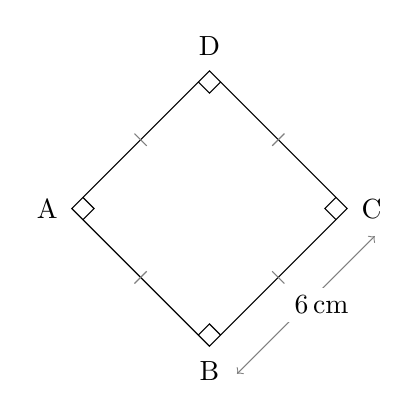
\begin{tikzpicture}[scale=1.1, baseline=(current bounding box.north)]
    \begin{scope}[rotate=-45]
        % Draw square
        \draw (0,0) coordinate (A) --
              ++(2.248,0) coordinate (B) --
              ++(0,2.248) coordinate (C) --
              ++(-2.248,0) coordinate (D) -- cycle;

        % Right angle markers
        \foreach \p/\q/\r in {D/A/B,A/B/C,B/C/D,C/D/A} {
            \pic [draw, -, angle radius=0.2cm] {right angle=\p--\q--\r};
        }

        % Vertex LABELS
        % Labels relative to shape geometry
        \node at ($(A)+(-0.2,-0.2)$) {A};
        \node at ($(B)+(0.2,-0.2)$) {B};
        \node at ($(C)+(0.2,0.2)$) {C};
        \node at ($(D)+(-0.2,0.2)$) {D};

        % Tick marks across horizontal sides
        \draw[thin, gray]
            ($(A)!0.5!(B) + (0,-0.10)$) --
            ($(A)!0.5!(B) + (0,0.10)$);

        \draw[thin, gray]
            ($(D)!0.5!(C) + (0,-0.10)$) --
            ($(D)!0.5!(C) + (0,0.10)$);

        % Tick marks across vertical sides
        \draw[thin, gray]
            ($(B)!0.5!(C) + (-0.10,0)$) --
            ($(B)!0.5!(C) + (0.10,0)$);

        \draw[thin, gray]
            ($(A)!0.5!(D) + (-0.10,0)$) --
            ($(A)!0.5!(D) + (0.10,0)$);


        % dotted/dashed arrows shifted away from edges
        % % Vertical side (B-C), shifted right
        \draw[<->, gray]
            ($(B) + (0.45cm,0)$) -- ($(C) + (0.45cm,0)$)
            node[black, midway, fill=white, xshift=2mm, inner sep=3pt] {6\,cm};

    \end{scope}
\end{tikzpicture}
\end{minipage}%
\hfill
\begin{minipage}{.4\textwidth}
  \begin{align*}
  \text{Area} &= l^2 \\
  \text{Area} &= \dotuline{~~~~~~~} \,\text{cm} \times \dotuline{~~~~~~~} \,\text{cm} \\
  \text{Area} &= \dotuline{~~~~~~~} \,\text{cm}^2
  \end{align*}
\end{minipage}
\par\vspace{1cm}\begin{minipage}{0.55\textwidth}
  \refstepcounter{minipagecount}
  \noindent{(\theminipagecount)}\quad
  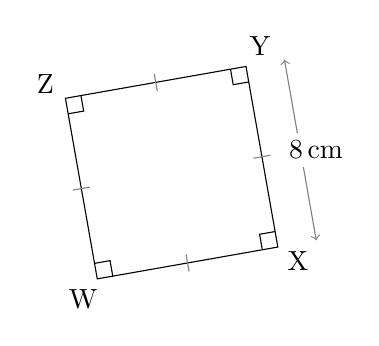
\begin{tikzpicture}[scale=1.1, baseline=(current bounding box.north)]
    \begin{scope}[rotate=10]
        % Draw square
        \draw (0,0) coordinate (W) --
              ++(2.117,0) coordinate (X) --
              ++(0,2.117) coordinate (Y) --
              ++(-2.117,0) coordinate (Z) -- cycle;

        % Right angle markers
        \foreach \p/\q/\r in {Z/W/X,W/X/Y,X/Y/Z,Y/Z/W} {
            \pic [draw, -, angle radius=0.2cm] {right angle=\p--\q--\r};
        }

        % Vertex LABELS
        % Labels relative to shape geometry
        \node at ($(W)+(-0.2,-0.2)$) {W};
        \node at ($(X)+(0.2,-0.2)$) {X};
        \node at ($(Y)+(0.2,0.2)$) {Y};
        \node at ($(Z)+(-0.2,0.2)$) {Z};

        % Tick marks across horizontal sides
        \draw[thin, gray]
            ($(W)!0.5!(X) + (0,-0.10)$) --
            ($(W)!0.5!(X) + (0,0.10)$);

        \draw[thin, gray]
            ($(Z)!0.5!(Y) + (0,-0.10)$) --
            ($(Z)!0.5!(Y) + (0,0.10)$);

        % Tick marks across vertical sides
        \draw[thin, gray]
            ($(X)!0.5!(Y) + (-0.10,0)$) --
            ($(X)!0.5!(Y) + (0.10,0)$);

        \draw[thin, gray]
            ($(W)!0.5!(Z) + (-0.10,0)$) --
            ($(W)!0.5!(Z) + (0.10,0)$);


        % dotted/dashed arrows shifted away from edges
        % % Vertical side (B-C), shifted right
        \draw[<->, gray]
            ($(X) + (0.45cm,0)$) -- ($(Y) + (0.45cm,0)$)
            node[black, midway, fill=white, xshift=2mm, inner sep=3pt] {8\,cm};

    \end{scope}
\end{tikzpicture}
\end{minipage}%
\hfill
\begin{minipage}{.4\textwidth}
  \begin{align*}
  \text{Area} &= l^2 \\
  \text{Area} &= \dotuline{~~~~~~~} \,\text{cm} \times \dotuline{~~~~~~~} \,\text{cm} \\
  \text{Area} &= \dotuline{~~~~~~~} \,\text{cm}^2
  \end{align*}
\end{minipage}
\par\vspace{1cm}\begin{minipage}{0.55\textwidth}
  \refstepcounter{minipagecount}
  \noindent{(\theminipagecount)}\quad
  \begin{tikzpicture}[scale=1.1, baseline=(current bounding box.north)]
    \begin{scope}[rotate=0]
        % Draw square
        \draw (0,0) coordinate (E) --
              ++(2.006,0) coordinate (F) --
              ++(0,2.006) coordinate (G) --
              ++(-2.006,0) coordinate (H) -- cycle;

        % Right angle markers
        \foreach \p/\q/\r in {H/E/F,E/F/G,F/G/H,G/H/E} {
            \pic [draw, -, angle radius=0.2cm] {right angle=\p--\q--\r};
        }

        % Vertex LABELS
        % Labels relative to shape geometry
        \node at ($(E)+(-0.2,-0.2)$) {E};
        \node at ($(F)+(0.2,-0.2)$) {F};
        \node at ($(G)+(0.2,0.2)$) {G};
        \node at ($(H)+(-0.2,0.2)$) {H};

        % Tick marks across horizontal sides
        \draw[thin, gray]
            ($(E)!0.5!(F) + (0,-0.10)$) --
            ($(E)!0.5!(F) + (0,0.10)$);

        \draw[thin, gray]
            ($(H)!0.5!(G) + (0,-0.10)$) --
            ($(H)!0.5!(G) + (0,0.10)$);

        % Tick marks across vertical sides
        \draw[thin, gray]
            ($(F)!0.5!(G) + (-0.10,0)$) --
            ($(F)!0.5!(G) + (0.10,0)$);

        \draw[thin, gray]
            ($(E)!0.5!(H) + (-0.10,0)$) --
            ($(E)!0.5!(H) + (0.10,0)$);


        % dotted/dashed arrows shifted away from edges
        % % Vertical side (B-C), shifted right
        \draw[<->, gray]
            ($(F) + (0.45cm,0)$) -- ($(G) + (0.45cm,0)$)
            node[black, midway, fill=white, xshift=2mm, inner sep=3pt] {3\,cm};

    \end{scope}
\end{tikzpicture}
\end{minipage}%
\hfill
\begin{minipage}{.4\textwidth}
  \begin{align*}
  \text{Area} &= l^2 \\
  \text{Area} &= \dotuline{~~~~~~~} \,\text{cm} \times \dotuline{~~~~~~~} \,\text{cm} \\
  \text{Area} &= \dotuline{~~~~~~~} \,\text{cm}^2
  \end{align*}
\end{minipage}
\par\vspace{1cm}\begin{minipage}{0.55\textwidth}
  \refstepcounter{minipagecount}
  \noindent{(\theminipagecount)}\quad
  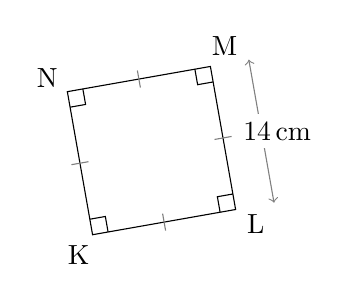
\begin{tikzpicture}[scale=1.1, baseline=(current bounding box.north)]
    \begin{scope}[rotate=10]
        % Draw square
        \draw (0,0) coordinate (K) --
              ++(1.677,0) coordinate (L) --
              ++(0,1.677) coordinate (M) --
              ++(-1.677,0) coordinate (N) -- cycle;

        % Right angle markers
        \foreach \p/\q/\r in {N/K/L,K/L/M,L/M/N,M/N/K} {
            \pic [draw, -, angle radius=0.2cm] {right angle=\p--\q--\r};
        }

        % Vertex LABELS
        % Labels relative to shape geometry
        \node at ($(K)+(-0.2,-0.2)$) {K};
        \node at ($(L)+(0.2,-0.2)$) {L};
        \node at ($(M)+(0.2,0.2)$) {M};
        \node at ($(N)+(-0.2,0.2)$) {N};

        % Tick marks across horizontal sides
        \draw[thin, gray]
            ($(K)!0.5!(L) + (0,-0.10)$) --
            ($(K)!0.5!(L) + (0,0.10)$);

        \draw[thin, gray]
            ($(N)!0.5!(M) + (0,-0.10)$) --
            ($(N)!0.5!(M) + (0,0.10)$);

        % Tick marks across vertical sides
        \draw[thin, gray]
            ($(L)!0.5!(M) + (-0.10,0)$) --
            ($(L)!0.5!(M) + (0.10,0)$);

        \draw[thin, gray]
            ($(K)!0.5!(N) + (-0.10,0)$) --
            ($(K)!0.5!(N) + (0.10,0)$);


        % dotted/dashed arrows shifted away from edges
        % % Vertical side (B-C), shifted right
        \draw[<->, gray]
            ($(L) + (0.45cm,0)$) -- ($(M) + (0.45cm,0)$)
            node[black, midway, fill=white, xshift=2mm, inner sep=3pt] {14\,cm};

    \end{scope}
\end{tikzpicture}
\end{minipage}%
\hfill
\begin{minipage}{.4\textwidth}
  \begin{align*}
  \text{Area} &= l^2 \\
  \text{Area} &= \dotuline{~~~~~~~} \,\text{cm} \times \dotuline{~~~~~~~} \,\text{cm} \\
  \text{Area} &= \dotuline{~~~~~~~} \,\text{cm}^2
  \end{align*}
\end{minipage}
\par\vspace{1cm}\begin{minipage}{0.55\textwidth}
  \refstepcounter{minipagecount}
  \noindent{(\theminipagecount)}\quad
  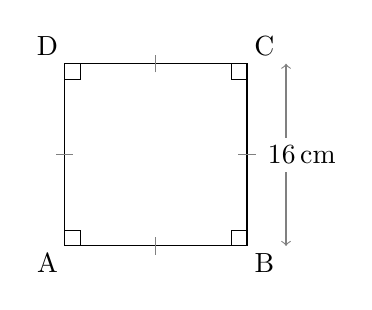
\begin{tikzpicture}[scale=1.1, baseline=(current bounding box.north)]
    \begin{scope}[rotate=0]
        % Draw square
        \draw (0,0) coordinate (A) --
              ++(2.104,0) coordinate (B) --
              ++(0,2.104) coordinate (C) --
              ++(-2.104,0) coordinate (D) -- cycle;

        % Right angle markers
        \foreach \p/\q/\r in {D/A/B,A/B/C,B/C/D,C/D/A} {
            \pic [draw, -, angle radius=0.2cm] {right angle=\p--\q--\r};
        }

        % Vertex LABELS
        % Labels relative to shape geometry
        \node at ($(A)+(-0.2,-0.2)$) {A};
        \node at ($(B)+(0.2,-0.2)$) {B};
        \node at ($(C)+(0.2,0.2)$) {C};
        \node at ($(D)+(-0.2,0.2)$) {D};

        % Tick marks across horizontal sides
        \draw[thin, gray]
            ($(A)!0.5!(B) + (0,-0.10)$) --
            ($(A)!0.5!(B) + (0,0.10)$);

        \draw[thin, gray]
            ($(D)!0.5!(C) + (0,-0.10)$) --
            ($(D)!0.5!(C) + (0,0.10)$);

        % Tick marks across vertical sides
        \draw[thin, gray]
            ($(B)!0.5!(C) + (-0.10,0)$) --
            ($(B)!0.5!(C) + (0.10,0)$);

        \draw[thin, gray]
            ($(A)!0.5!(D) + (-0.10,0)$) --
            ($(A)!0.5!(D) + (0.10,0)$);


        % dotted/dashed arrows shifted away from edges
        % % Vertical side (B-C), shifted right
        \draw[<->, gray]
            ($(B) + (0.45cm,0)$) -- ($(C) + (0.45cm,0)$)
            node[black, midway, fill=white, xshift=2mm, inner sep=3pt] {16\,cm};

    \end{scope}
\end{tikzpicture}
\end{minipage}%
\hfill
\begin{minipage}{.4\textwidth}
  \begin{align*}
  \text{Area} &= l^2 \\
  \text{Area} &= \dotuline{~~~~~~~} \,\text{cm} \times \dotuline{~~~~~~~} \,\text{cm} \\
  \text{Area} &= \dotuline{~~~~~~~} \,\text{cm}^2
  \end{align*}
\end{minipage}
\par\vspace{1cm}\begin{minipage}{0.55\textwidth}
  \refstepcounter{minipagecount}
  \noindent{(\theminipagecount)}\quad
  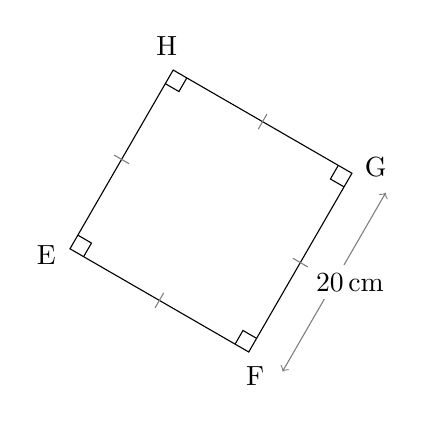
\begin{tikzpicture}[scale=1.1, baseline=(current bounding box.north)]
    \begin{scope}[rotate=-30]
        % Draw square
        \draw (0,0) coordinate (E) --
              ++(2.383,0) coordinate (F) --
              ++(0,2.383) coordinate (G) --
              ++(-2.383,0) coordinate (H) -- cycle;

        % Right angle markers
        \foreach \p/\q/\r in {H/E/F,E/F/G,F/G/H,G/H/E} {
            \pic [draw, -, angle radius=0.2cm] {right angle=\p--\q--\r};
        }

        % Vertex LABELS
        % Labels relative to shape geometry
        \node at ($(E)+(-0.2,-0.2)$) {E};
        \node at ($(F)+(0.2,-0.2)$) {F};
        \node at ($(G)+(0.2,0.2)$) {G};
        \node at ($(H)+(-0.2,0.2)$) {H};

        % Tick marks across horizontal sides
        \draw[thin, gray]
            ($(E)!0.5!(F) + (0,-0.10)$) --
            ($(E)!0.5!(F) + (0,0.10)$);

        \draw[thin, gray]
            ($(H)!0.5!(G) + (0,-0.10)$) --
            ($(H)!0.5!(G) + (0,0.10)$);

        % Tick marks across vertical sides
        \draw[thin, gray]
            ($(F)!0.5!(G) + (-0.10,0)$) --
            ($(F)!0.5!(G) + (0.10,0)$);

        \draw[thin, gray]
            ($(E)!0.5!(H) + (-0.10,0)$) --
            ($(E)!0.5!(H) + (0.10,0)$);


        % dotted/dashed arrows shifted away from edges
        % % Vertical side (B-C), shifted right
        \draw[<->, gray]
            ($(F) + (0.45cm,0)$) -- ($(G) + (0.45cm,0)$)
            node[black, midway, fill=white, xshift=2mm, inner sep=3pt] {20\,cm};

    \end{scope}
\end{tikzpicture}
\end{minipage}%
\hfill
\begin{minipage}{.4\textwidth}
  \begin{align*}
  \text{Area} &= l^2 \\
  \text{Area} &= \dotuline{~~~~~~~} \,\text{cm} \times \dotuline{~~~~~~~} \,\text{cm} \\
  \text{Area} &= \dotuline{~~~~~~~} \,\text{cm}^2
  \end{align*}
\end{minipage}
\par\vspace{1cm}\begin{minipage}{0.55\textwidth}
  \refstepcounter{minipagecount}
  \noindent{(\theminipagecount)}\quad
  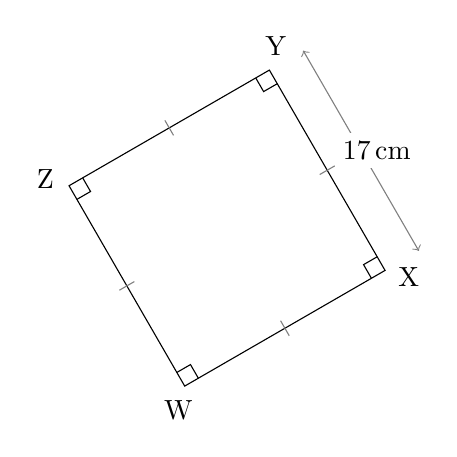
\begin{tikzpicture}[scale=1.1, baseline=(current bounding box.north)]
    \begin{scope}[rotate=30]
        % Draw square
        \draw (0,0) coordinate (W) --
              ++(2.671,0) coordinate (X) --
              ++(0,2.671) coordinate (Y) --
              ++(-2.671,0) coordinate (Z) -- cycle;

        % Right angle markers
        \foreach \p/\q/\r in {Z/W/X,W/X/Y,X/Y/Z,Y/Z/W} {
            \pic [draw, -, angle radius=0.2cm] {right angle=\p--\q--\r};
        }

        % Vertex LABELS
        % Labels relative to shape geometry
        \node at ($(W)+(-0.2,-0.2)$) {W};
        \node at ($(X)+(0.2,-0.2)$) {X};
        \node at ($(Y)+(0.2,0.2)$) {Y};
        \node at ($(Z)+(-0.2,0.2)$) {Z};

        % Tick marks across horizontal sides
        \draw[thin, gray]
            ($(W)!0.5!(X) + (0,-0.10)$) --
            ($(W)!0.5!(X) + (0,0.10)$);

        \draw[thin, gray]
            ($(Z)!0.5!(Y) + (0,-0.10)$) --
            ($(Z)!0.5!(Y) + (0,0.10)$);

        % Tick marks across vertical sides
        \draw[thin, gray]
            ($(X)!0.5!(Y) + (-0.10,0)$) --
            ($(X)!0.5!(Y) + (0.10,0)$);

        \draw[thin, gray]
            ($(W)!0.5!(Z) + (-0.10,0)$) --
            ($(W)!0.5!(Z) + (0.10,0)$);


        % dotted/dashed arrows shifted away from edges
        % % Vertical side (B-C), shifted right
        \draw[<->, gray]
            ($(X) + (0.45cm,0)$) -- ($(Y) + (0.45cm,0)$)
            node[black, midway, fill=white, xshift=2mm, inner sep=3pt] {17\,cm};

    \end{scope}
\end{tikzpicture}
\end{minipage}%
\hfill
\begin{minipage}{.4\textwidth}
  \begin{align*}
  \text{Area} &= l^2 \\
  \text{Area} &= \dotuline{~~~~~~~} \,\text{cm} \times \dotuline{~~~~~~~} \,\text{cm} \\
  \text{Area} &= \dotuline{~~~~~~~} \,\text{cm}^2
  \end{align*}
\end{minipage}
\par\vspace{1cm}\begin{minipage}{0.55\textwidth}
  \refstepcounter{minipagecount}
  \noindent{(\theminipagecount)}\quad
  \begin{tikzpicture}[scale=1.1, baseline=(current bounding box.north)]
    \begin{scope}[rotate=0]
        % Draw square
        \draw (0,0) coordinate (W) --
              ++(2.595,0) coordinate (X) --
              ++(0,2.595) coordinate (Y) --
              ++(-2.595,0) coordinate (Z) -- cycle;

        % Right angle markers
        \foreach \p/\q/\r in {Z/W/X,W/X/Y,X/Y/Z,Y/Z/W} {
            \pic [draw, -, angle radius=0.2cm] {right angle=\p--\q--\r};
        }

        % Vertex LABELS
        % Labels relative to shape geometry
        \node at ($(W)+(-0.2,-0.2)$) {W};
        \node at ($(X)+(0.2,-0.2)$) {X};
        \node at ($(Y)+(0.2,0.2)$) {Y};
        \node at ($(Z)+(-0.2,0.2)$) {Z};

        % Tick marks across horizontal sides
        \draw[thin, gray]
            ($(W)!0.5!(X) + (0,-0.10)$) --
            ($(W)!0.5!(X) + (0,0.10)$);

        \draw[thin, gray]
            ($(Z)!0.5!(Y) + (0,-0.10)$) --
            ($(Z)!0.5!(Y) + (0,0.10)$);

        % Tick marks across vertical sides
        \draw[thin, gray]
            ($(X)!0.5!(Y) + (-0.10,0)$) --
            ($(X)!0.5!(Y) + (0.10,0)$);

        \draw[thin, gray]
            ($(W)!0.5!(Z) + (-0.10,0)$) --
            ($(W)!0.5!(Z) + (0.10,0)$);


        % dotted/dashed arrows shifted away from edges
        % % Vertical side (B-C), shifted right
        \draw[<->, gray]
            ($(X) + (0.45cm,0)$) -- ($(Y) + (0.45cm,0)$)
            node[black, midway, fill=white, xshift=2mm, inner sep=3pt] {18\,cm};

    \end{scope}
\end{tikzpicture}
\end{minipage}%
\hfill
\begin{minipage}{.4\textwidth}
  \begin{align*}
  \text{Area} &= l^2 \\
  \text{Area} &= \dotuline{~~~~~~~} \,\text{cm} \times \dotuline{~~~~~~~} \,\text{cm} \\
  \text{Area} &= \dotuline{~~~~~~~} \,\text{cm}^2
  \end{align*}
\end{minipage}
\par\vspace{1cm}\begin{minipage}{0.55\textwidth}
  \refstepcounter{minipagecount}
  \noindent{(\theminipagecount)}\quad
  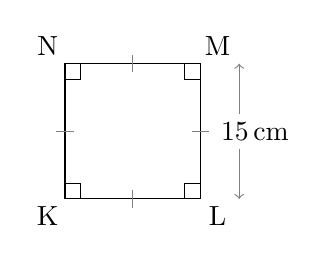
\begin{tikzpicture}[scale=1.1, baseline=(current bounding box.north)]
    \begin{scope}[rotate=0]
        % Draw square
        \draw (0,0) coordinate (K) --
              ++(1.561,0) coordinate (L) --
              ++(0,1.561) coordinate (M) --
              ++(-1.561,0) coordinate (N) -- cycle;

        % Right angle markers
        \foreach \p/\q/\r in {N/K/L,K/L/M,L/M/N,M/N/K} {
            \pic [draw, -, angle radius=0.2cm] {right angle=\p--\q--\r};
        }

        % Vertex LABELS
        % Labels relative to shape geometry
        \node at ($(K)+(-0.2,-0.2)$) {K};
        \node at ($(L)+(0.2,-0.2)$) {L};
        \node at ($(M)+(0.2,0.2)$) {M};
        \node at ($(N)+(-0.2,0.2)$) {N};

        % Tick marks across horizontal sides
        \draw[thin, gray]
            ($(K)!0.5!(L) + (0,-0.10)$) --
            ($(K)!0.5!(L) + (0,0.10)$);

        \draw[thin, gray]
            ($(N)!0.5!(M) + (0,-0.10)$) --
            ($(N)!0.5!(M) + (0,0.10)$);

        % Tick marks across vertical sides
        \draw[thin, gray]
            ($(L)!0.5!(M) + (-0.10,0)$) --
            ($(L)!0.5!(M) + (0.10,0)$);

        \draw[thin, gray]
            ($(K)!0.5!(N) + (-0.10,0)$) --
            ($(K)!0.5!(N) + (0.10,0)$);


        % dotted/dashed arrows shifted away from edges
        % % Vertical side (B-C), shifted right
        \draw[<->, gray]
            ($(L) + (0.45cm,0)$) -- ($(M) + (0.45cm,0)$)
            node[black, midway, fill=white, xshift=2mm, inner sep=3pt] {15\,cm};

    \end{scope}
\end{tikzpicture}
\end{minipage}%
\hfill
\begin{minipage}{.4\textwidth}
  \begin{align*}
  \text{Area} &= l^2 \\
  \text{Area} &= \dotuline{~~~~~~~} \,\text{cm} \times \dotuline{~~~~~~~} \,\text{cm} \\
  \text{Area} &= \dotuline{~~~~~~~} \,\text{cm}^2
  \end{align*}
\end{minipage}
\par\vspace{1cm}\begin{minipage}{0.55\textwidth}
  \refstepcounter{minipagecount}
  \noindent{(\theminipagecount)}\quad
  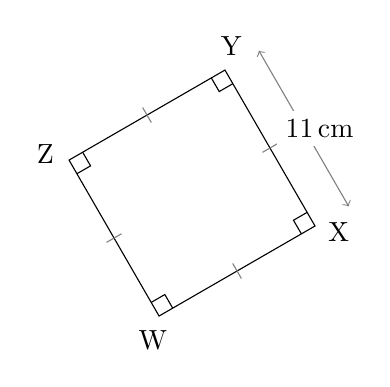
\begin{tikzpicture}[scale=1.1, baseline=(current bounding box.north)]
    \begin{scope}[rotate=30]
        % Draw square
        \draw (0,0) coordinate (W) --
              ++(2.079,0) coordinate (X) --
              ++(0,2.079) coordinate (Y) --
              ++(-2.079,0) coordinate (Z) -- cycle;

        % Right angle markers
        \foreach \p/\q/\r in {Z/W/X,W/X/Y,X/Y/Z,Y/Z/W} {
            \pic [draw, -, angle radius=0.2cm] {right angle=\p--\q--\r};
        }

        % Vertex LABELS
        % Labels relative to shape geometry
        \node at ($(W)+(-0.2,-0.2)$) {W};
        \node at ($(X)+(0.2,-0.2)$) {X};
        \node at ($(Y)+(0.2,0.2)$) {Y};
        \node at ($(Z)+(-0.2,0.2)$) {Z};

        % Tick marks across horizontal sides
        \draw[thin, gray]
            ($(W)!0.5!(X) + (0,-0.10)$) --
            ($(W)!0.5!(X) + (0,0.10)$);

        \draw[thin, gray]
            ($(Z)!0.5!(Y) + (0,-0.10)$) --
            ($(Z)!0.5!(Y) + (0,0.10)$);

        % Tick marks across vertical sides
        \draw[thin, gray]
            ($(X)!0.5!(Y) + (-0.10,0)$) --
            ($(X)!0.5!(Y) + (0.10,0)$);

        \draw[thin, gray]
            ($(W)!0.5!(Z) + (-0.10,0)$) --
            ($(W)!0.5!(Z) + (0.10,0)$);


        % dotted/dashed arrows shifted away from edges
        % % Vertical side (B-C), shifted right
        \draw[<->, gray]
            ($(X) + (0.45cm,0)$) -- ($(Y) + (0.45cm,0)$)
            node[black, midway, fill=white, xshift=2mm, inner sep=3pt] {11\,cm};

    \end{scope}
\end{tikzpicture}
\end{minipage}%
\hfill
\begin{minipage}{.4\textwidth}
  \begin{align*}
  \text{Area} &= l^2 \\
  \text{Area} &= \dotuline{~~~~~~~} \,\text{cm} \times \dotuline{~~~~~~~} \,\text{cm} \\
  \text{Area} &= \dotuline{~~~~~~~} \,\text{cm}^2
  \end{align*}
\end{minipage}
\par\vspace{1cm}\begin{minipage}{0.55\textwidth}
  \refstepcounter{minipagecount}
  \noindent{(\theminipagecount)}\quad
  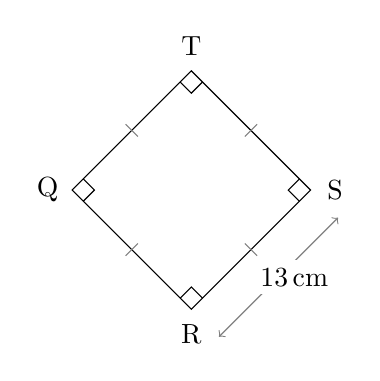
\begin{tikzpicture}[scale=1.1, baseline=(current bounding box.north)]
    \begin{scope}[rotate=-45]
        % Draw square
        \draw (0,0) coordinate (Q) --
              ++(1.946,0) coordinate (R) --
              ++(0,1.946) coordinate (S) --
              ++(-1.946,0) coordinate (T) -- cycle;

        % Right angle markers
        \foreach \p/\q/\r in {T/Q/R,Q/R/S,R/S/T,S/T/Q} {
            \pic [draw, -, angle radius=0.2cm] {right angle=\p--\q--\r};
        }

        % Vertex LABELS
        % Labels relative to shape geometry
        \node at ($(Q)+(-0.2,-0.2)$) {Q};
        \node at ($(R)+(0.2,-0.2)$) {R};
        \node at ($(S)+(0.2,0.2)$) {S};
        \node at ($(T)+(-0.2,0.2)$) {T};

        % Tick marks across horizontal sides
        \draw[thin, gray]
            ($(Q)!0.5!(R) + (0,-0.10)$) --
            ($(Q)!0.5!(R) + (0,0.10)$);

        \draw[thin, gray]
            ($(T)!0.5!(S) + (0,-0.10)$) --
            ($(T)!0.5!(S) + (0,0.10)$);

        % Tick marks across vertical sides
        \draw[thin, gray]
            ($(R)!0.5!(S) + (-0.10,0)$) --
            ($(R)!0.5!(S) + (0.10,0)$);

        \draw[thin, gray]
            ($(Q)!0.5!(T) + (-0.10,0)$) --
            ($(Q)!0.5!(T) + (0.10,0)$);


        % dotted/dashed arrows shifted away from edges
        % % Vertical side (B-C), shifted right
        \draw[<->, gray]
            ($(R) + (0.45cm,0)$) -- ($(S) + (0.45cm,0)$)
            node[black, midway, fill=white, xshift=2mm, inner sep=3pt] {13\,cm};

    \end{scope}
\end{tikzpicture}
\end{minipage}%
\hfill
\begin{minipage}{.4\textwidth}
  \begin{align*}
  \text{Area} &= l^2 \\
  \text{Area} &= \dotuline{~~~~~~~} \,\text{cm} \times \dotuline{~~~~~~~} \,\text{cm} \\
  \text{Area} &= \dotuline{~~~~~~~} \,\text{cm}^2
  \end{align*}
\end{minipage}
\par\vspace{1cm}\begin{minipage}{0.55\textwidth}
  \refstepcounter{minipagecount}
  \noindent{(\theminipagecount)}\quad
  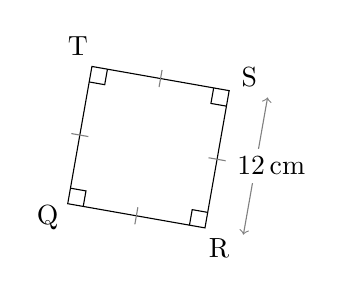
\begin{tikzpicture}[scale=1.1, baseline=(current bounding box.north)]
    \begin{scope}[rotate=-10]
        % Draw square
        \draw (0,0) coordinate (Q) --
              ++(1.609,0) coordinate (R) --
              ++(0,1.609) coordinate (S) --
              ++(-1.609,0) coordinate (T) -- cycle;

        % Right angle markers
        \foreach \p/\q/\r in {T/Q/R,Q/R/S,R/S/T,S/T/Q} {
            \pic [draw, -, angle radius=0.2cm] {right angle=\p--\q--\r};
        }

        % Vertex LABELS
        % Labels relative to shape geometry
        \node at ($(Q)+(-0.2,-0.2)$) {Q};
        \node at ($(R)+(0.2,-0.2)$) {R};
        \node at ($(S)+(0.2,0.2)$) {S};
        \node at ($(T)+(-0.2,0.2)$) {T};

        % Tick marks across horizontal sides
        \draw[thin, gray]
            ($(Q)!0.5!(R) + (0,-0.10)$) --
            ($(Q)!0.5!(R) + (0,0.10)$);

        \draw[thin, gray]
            ($(T)!0.5!(S) + (0,-0.10)$) --
            ($(T)!0.5!(S) + (0,0.10)$);

        % Tick marks across vertical sides
        \draw[thin, gray]
            ($(R)!0.5!(S) + (-0.10,0)$) --
            ($(R)!0.5!(S) + (0.10,0)$);

        \draw[thin, gray]
            ($(Q)!0.5!(T) + (-0.10,0)$) --
            ($(Q)!0.5!(T) + (0.10,0)$);


        % dotted/dashed arrows shifted away from edges
        % % Vertical side (B-C), shifted right
        \draw[<->, gray]
            ($(R) + (0.45cm,0)$) -- ($(S) + (0.45cm,0)$)
            node[black, midway, fill=white, xshift=2mm, inner sep=3pt] {12\,cm};

    \end{scope}
\end{tikzpicture}
\end{minipage}%
\hfill
\begin{minipage}{.4\textwidth}
  \begin{align*}
  \text{Area} &= l^2 \\
  \text{Area} &= \dotuline{~~~~~~~} \,\text{cm} \times \dotuline{~~~~~~~} \,\text{cm} \\
  \text{Area} &= \dotuline{~~~~~~~} \,\text{cm}^2
  \end{align*}
\end{minipage}
\par\vspace{1cm}\begin{minipage}{0.55\textwidth}
  \refstepcounter{minipagecount}
  \noindent{(\theminipagecount)}\quad
  \begin{tikzpicture}[scale=1.1, baseline=(current bounding box.north)]
    \begin{scope}[rotate=0]
        % Draw square
        \draw (0,0) coordinate (K) --
              ++(2.772,0) coordinate (L) --
              ++(0,2.772) coordinate (M) --
              ++(-2.772,0) coordinate (N) -- cycle;

        % Right angle markers
        \foreach \p/\q/\r in {N/K/L,K/L/M,L/M/N,M/N/K} {
            \pic [draw, -, angle radius=0.2cm] {right angle=\p--\q--\r};
        }

        % Vertex LABELS
        % Labels relative to shape geometry
        \node at ($(K)+(-0.2,-0.2)$) {K};
        \node at ($(L)+(0.2,-0.2)$) {L};
        \node at ($(M)+(0.2,0.2)$) {M};
        \node at ($(N)+(-0.2,0.2)$) {N};

        % Tick marks across horizontal sides
        \draw[thin, gray]
            ($(K)!0.5!(L) + (0,-0.10)$) --
            ($(K)!0.5!(L) + (0,0.10)$);

        \draw[thin, gray]
            ($(N)!0.5!(M) + (0,-0.10)$) --
            ($(N)!0.5!(M) + (0,0.10)$);

        % Tick marks across vertical sides
        \draw[thin, gray]
            ($(L)!0.5!(M) + (-0.10,0)$) --
            ($(L)!0.5!(M) + (0.10,0)$);

        \draw[thin, gray]
            ($(K)!0.5!(N) + (-0.10,0)$) --
            ($(K)!0.5!(N) + (0.10,0)$);


        % dotted/dashed arrows shifted away from edges
        % % Vertical side (B-C), shifted right
        \draw[<->, gray]
            ($(L) + (0.45cm,0)$) -- ($(M) + (0.45cm,0)$)
            node[black, midway, fill=white, xshift=2mm, inner sep=3pt] {19\,cm};

    \end{scope}
\end{tikzpicture}
\end{minipage}%
\hfill
\begin{minipage}{.4\textwidth}
  \begin{align*}
  \text{Area} &= l^2 \\
  \text{Area} &= \dotuline{~~~~~~~} \,\text{cm} \times \dotuline{~~~~~~~} \,\text{cm} \\
  \text{Area} &= \dotuline{~~~~~~~} \,\text{cm}^2
  \end{align*}
\end{minipage}
\par\vspace{1cm}\begin{minipage}{0.55\textwidth}
  \refstepcounter{minipagecount}
  \noindent{(\theminipagecount)}\quad
  \begin{tikzpicture}[scale=1.1, baseline=(current bounding box.north)]
    \begin{scope}[rotate=0]
        % Draw square
        \draw (0,0) coordinate (W) --
              ++(2.736,0) coordinate (X) --
              ++(0,2.736) coordinate (Y) --
              ++(-2.736,0) coordinate (Z) -- cycle;

        % Right angle markers
        \foreach \p/\q/\r in {Z/W/X,W/X/Y,X/Y/Z,Y/Z/W} {
            \pic [draw, -, angle radius=0.2cm] {right angle=\p--\q--\r};
        }

        % Vertex LABELS
        % Labels relative to shape geometry
        \node at ($(W)+(-0.2,-0.2)$) {W};
        \node at ($(X)+(0.2,-0.2)$) {X};
        \node at ($(Y)+(0.2,0.2)$) {Y};
        \node at ($(Z)+(-0.2,0.2)$) {Z};

        % Tick marks across horizontal sides
        \draw[thin, gray]
            ($(W)!0.5!(X) + (0,-0.10)$) --
            ($(W)!0.5!(X) + (0,0.10)$);

        \draw[thin, gray]
            ($(Z)!0.5!(Y) + (0,-0.10)$) --
            ($(Z)!0.5!(Y) + (0,0.10)$);

        % Tick marks across vertical sides
        \draw[thin, gray]
            ($(X)!0.5!(Y) + (-0.10,0)$) --
            ($(X)!0.5!(Y) + (0.10,0)$);

        \draw[thin, gray]
            ($(W)!0.5!(Z) + (-0.10,0)$) --
            ($(W)!0.5!(Z) + (0.10,0)$);


        % dotted/dashed arrows shifted away from edges
        % % Vertical side (B-C), shifted right
        \draw[<->, gray]
            ($(X) + (0.45cm,0)$) -- ($(Y) + (0.45cm,0)$)
            node[black, midway, fill=white, xshift=2mm, inner sep=3pt] {10\,cm};

    \end{scope}
\end{tikzpicture}
\end{minipage}%
\hfill
\begin{minipage}{.4\textwidth}
  \begin{align*}
  \text{Area} &= l^2 \\
  \text{Area} &= \dotuline{~~~~~~~} \,\text{cm} \times \dotuline{~~~~~~~} \,\text{cm} \\
  \text{Area} &= \dotuline{~~~~~~~} \,\text{cm}^2
  \end{align*}
\end{minipage}
\par\vspace{1cm}

\end{document}
